\chapter{Theory}
Small particles can be trapped in the focal point of a laser, held by radiation pressure.

Two models can be used to describe this effect, both depend on the laser beam having a gaussian intensity profile across its diameter.

\section{Geometrical Optics Model}
Geometrical optics only apply when the wavelength is much smaller than the feature size of the particles.
Also the particles are assumed to be roughly spherical.
In this case the laser beam can be split up into many parallel rays of light, which are refracted by the particles.
As the rays change direction at the boundaries, the photons transfer momentum to the particle, pushing it slightly towards the side where the ray hits the particle.
This is due to conservation of momentum, the photons leaving the particle have a different momentum than before entering the particle.
As the rays have lower intensities further away from the center of the beam, the force they impart on the particle is smaller and the particle experiences a net force towards the center of the beam.
\begin{figure}[bp]
  \centering
  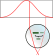
\includegraphics[width=.5\textwidth]{./img/geometrical-optics.pdf}
  \caption{Geometrical Optics Model}
\end{figure}

\section{Maxwell Model}
The above model only holds for large particles and small wavelengths.
For wavelengths that are of the same order as the particles themselves, a different model has to be considered.

The energy of a dielectric in an electric field is given by $U = -\vec{P}\vec{E}$.
For ''slow'' changing fields, the polarization is proportional to the electric field.
This results in an interaction energy of $U = -\Xi \vec{E}^2 \propto -I$ with the electric susceptibility $\Xi$ and the intensity of light $I$.

Due to the positive sign of $\Xi$ for small frequencies, the interaction energy of a particle in a beam with a gaussian intensity profile has a local minimum at the center, where intensity is highest.
The principle of minimum energy states that the particle lies in a stable state there. \todo{rephrase that}
